%!TEX program = xelatex
%!TEX TS-program = xelatex
%!TEX encoding = UTF-8 Unicode

\documentclass[a4paper]{article}
\usepackage[UTF8, heading = false, scheme = plain]{ctex}
\usepackage{graphicx}
\usepackage{cite}
\usepackage{geometry}
\geometry{left=2.0cm, right=2.0cm, top=2.5cm, bottom=2.5cm}
\usepackage[colorlinks,linkcolor=red,anchorcolor=blue,citecolor=green]{hyperref}
\usepackage{subfig}
\usepackage{caption}
\captionsetup{font={scriptsize}}

\renewcommand\figurename{图}

%%%% 段落首行缩进两个字 %%%%
\makeatletter
\let\@afterindentfalse\@afterindenttrue
\@afterindenttrue
\makeatother
\setlength{\parindent}{2em}  %中文缩进两个汉字位

%%%% 下面的命令设置行间距与段落间距 %%%%
\linespread{1.4}
% \setlength{\parskip}{1ex}
\setlength{\parskip}{0.5\baselineskip}

\title{学习汇报}
\author{熊凯亚}
\date{\today}

\begin{document}
\maketitle

\section{引言}

%最近两周看了一些关于去中心化深度学习中的隐私保护问题。如\cite{hitaj2017deep}中提出了一种攻击模型,这种模型针对于\cite{shokri2015privacy}中提出的协作学习进行了攻击。\cite{46432},\cite{abadi2016deep},\cite{bonawitz2017practical},\cite{Phong2017PrivacyPreservingDL}.

最近看了一些关于在去中心化的深度学习场景下的隐私保护的文章。去中心化的深度学习主要有两个方向,一是,CCS'15上Shokri等人\cite{shokri2015privacy}提出的隐私保护多方参与的协作深度学习模型(Collaborative Deep Learning);二是,Google 提出的针对移动设备(Android)的多方参与的\href{https://research.googleblog.com/2017/04/federated-learning-collaborative.html}{联合学习}(Federated Learning)。\\

\begin{figure*}[!ht]
\begin{tabular}{cc}
\subfloat[传统的中心化学习]{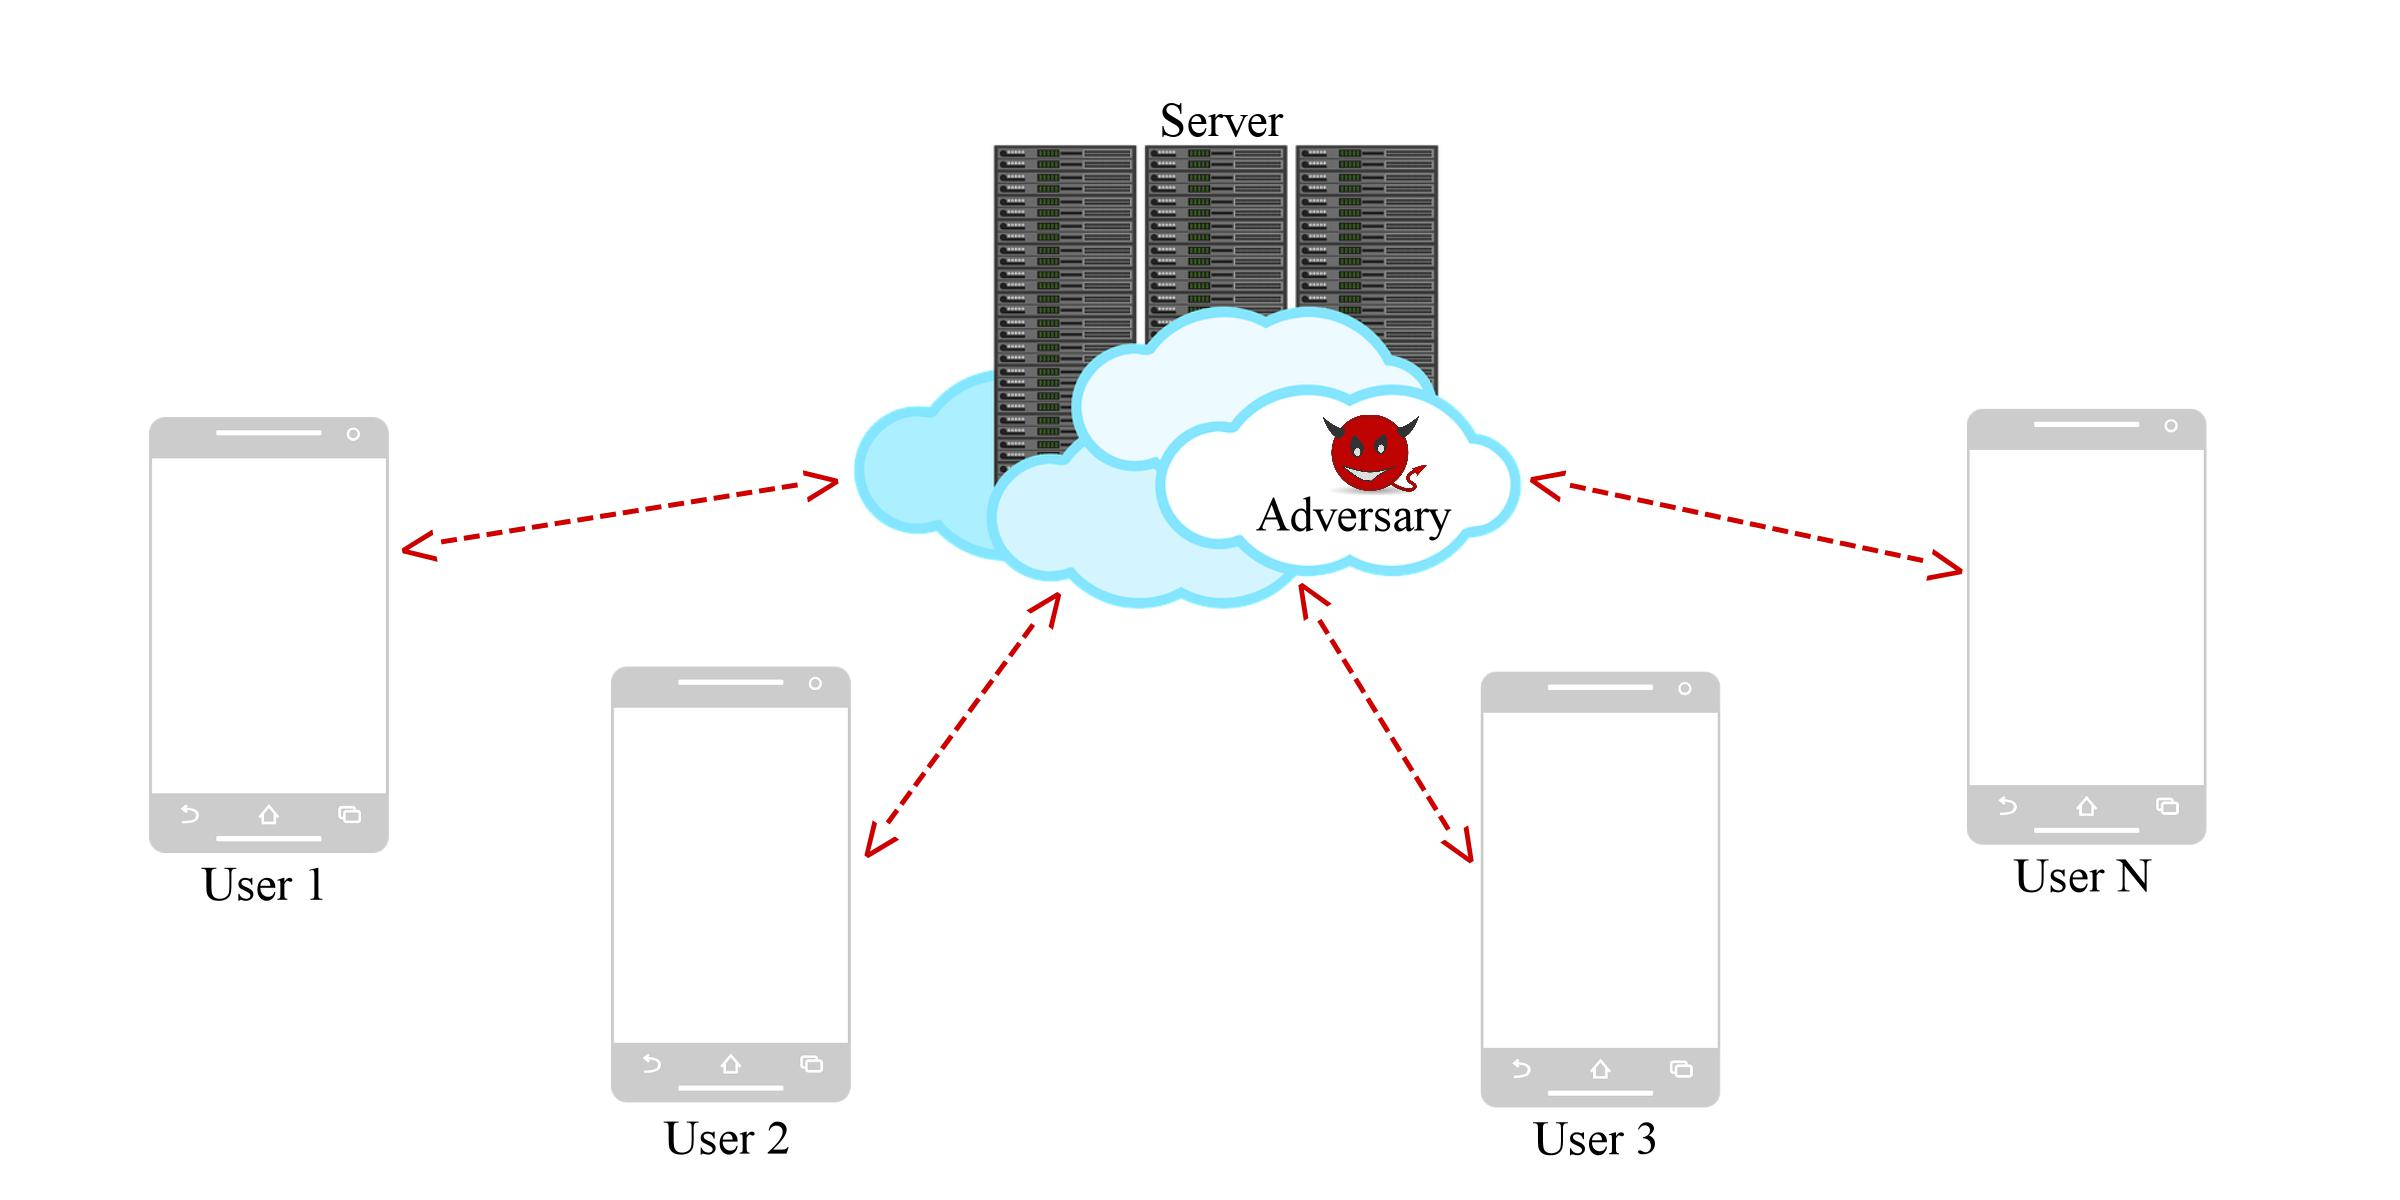
\includegraphics[width = 3.5in]{fig/scenario_1}} &
\subfloat[去中心化学习]{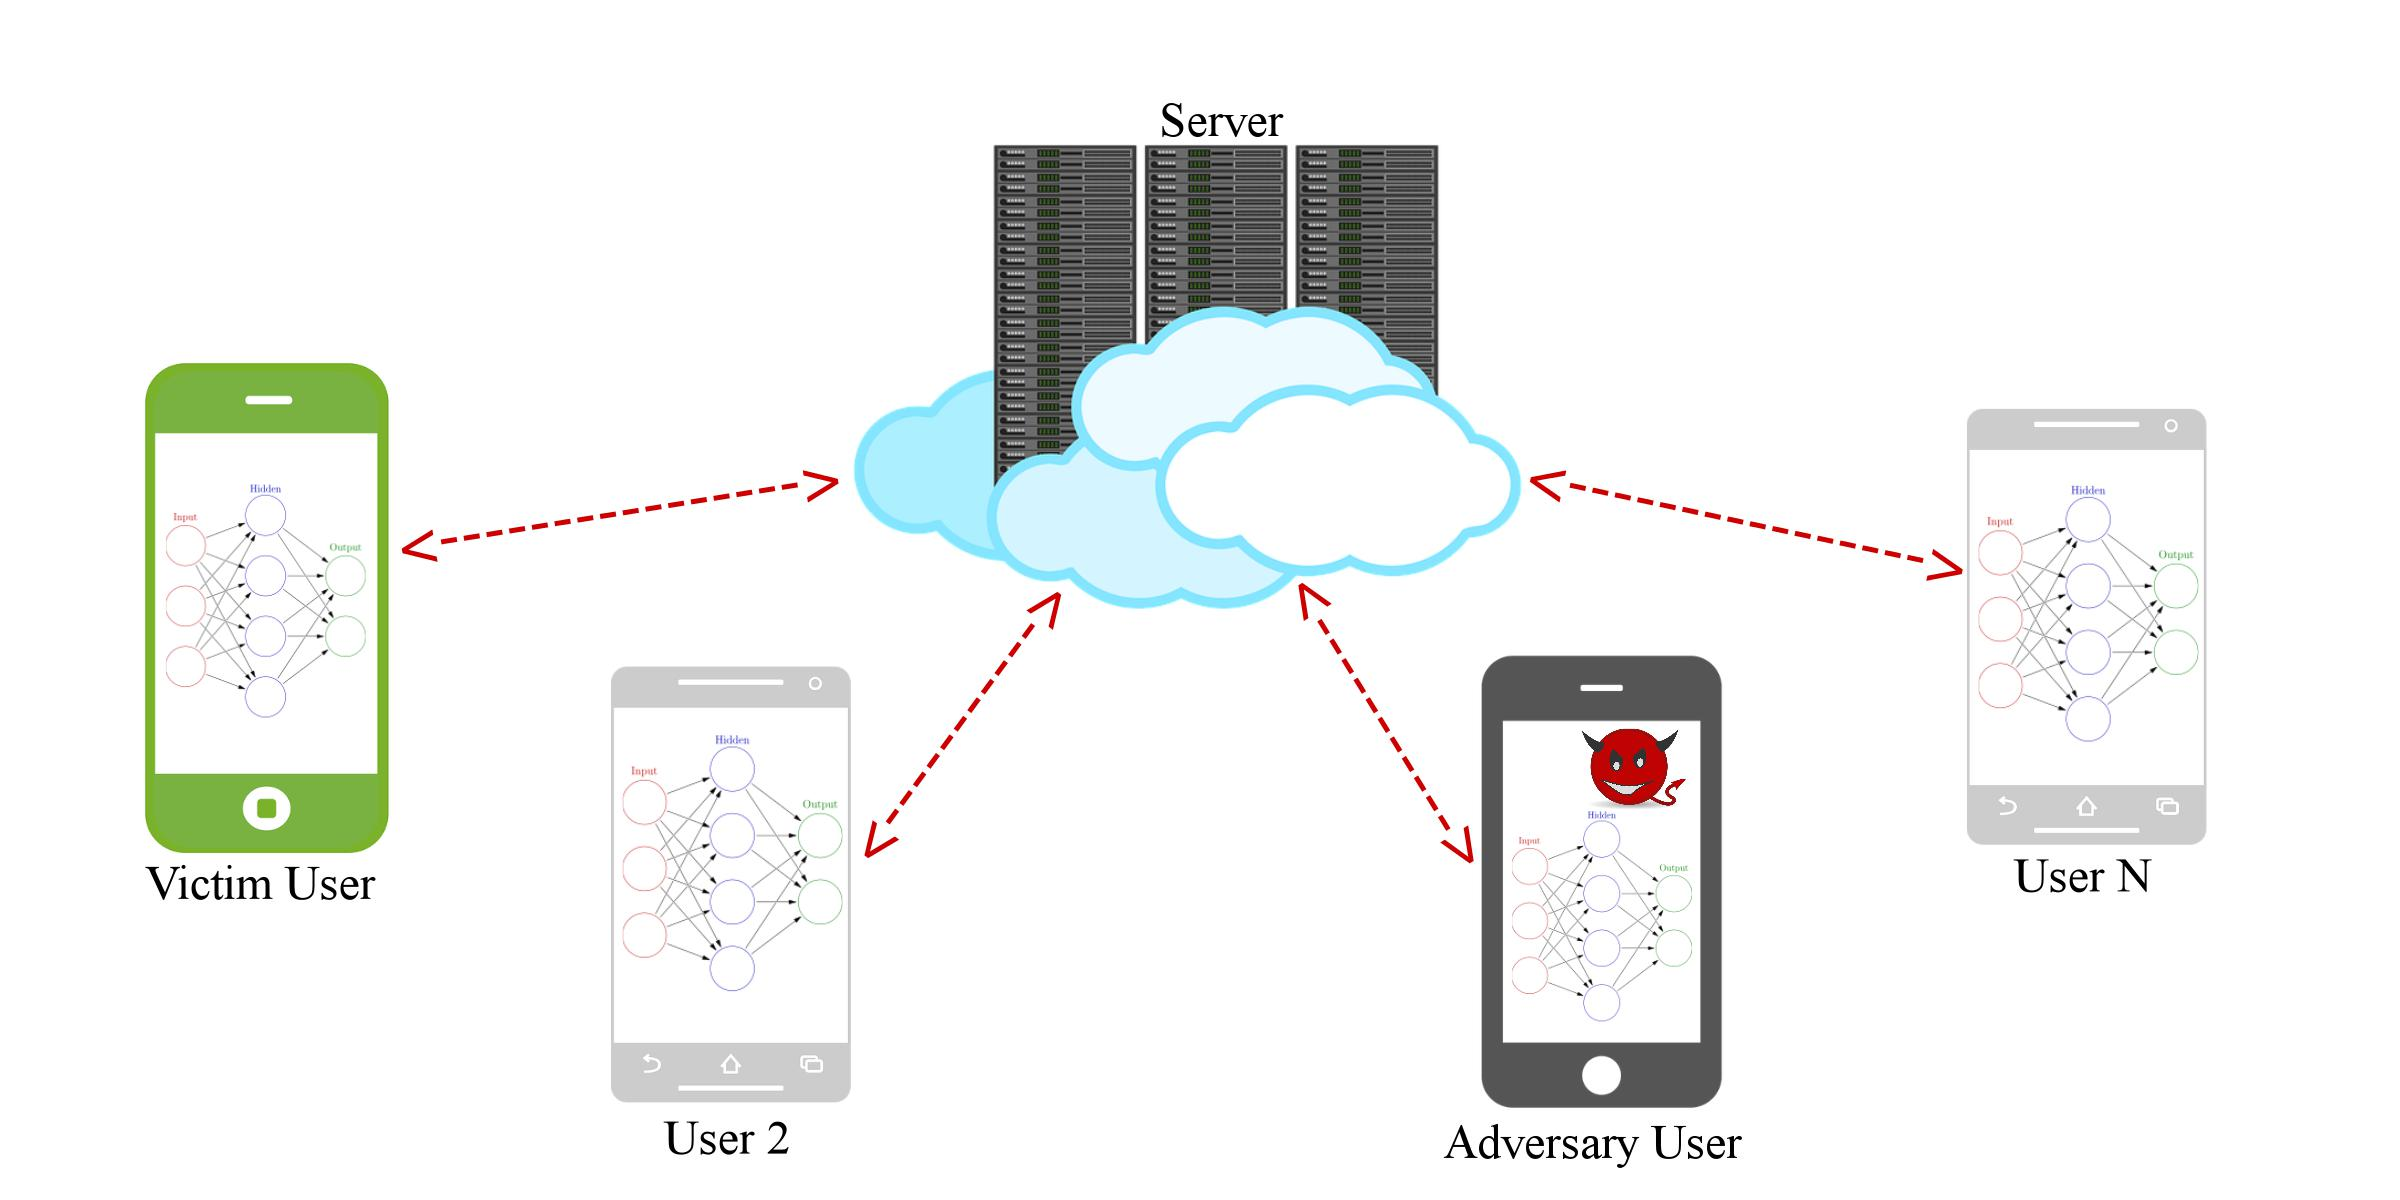
\includegraphics[width = 3.5in]{fig/scenario_2}}
\end{tabular}
\caption{传统中心化学习和去中心化学习对比}
\label{fig:learningApproaches}
\end{figure*}

在传统的中心化的深度学习模型中,用户将自己的数据(一部分是敏感数据)交给中心化的深度学习公司,对于这些数据,用户无法删除它,也无从知道这些公司怎样使用他们的这些数据,因此他们的他们的数据可能会面临隐私泄露的风险。而在去中心化的深度学习模型中,多个学习参与方可以共同训练一个模型,而不需要将他们的隐私数据集分享给别人。在\cite{shokri2015privacy}中提出的协作深度学习中(如图1b),每个参与方都可以独立地在本地训练他们的数据集,然后选择性地分享一小部分他们训练的模型的关键参数给一个中心化的参数服务器(Parameter Server),这样一方面可以保护参与者的敏感数据不被泄露,另一方面又可以从别的参与者分享的模型中收益,加速自己训练的模型的准确性。之后Google提出了联合学习的概念,在联合学习中,参与者在移动设备中存储所有的训练数据,在本地训练数据,然后将训练得到的更新(Updates)上传到云端,其他参与者下载更新到自己的移动设备,提高训练模型的准确性,利用这种方式联合学习解决了以前模型只能云端下发训练好的模型,而无法在本地训练的问题。联合学习的过程为:移动设备下载云端最新的共享模型,根据移动设备上用户的历史数据来改进和训练这个模型,然后将用户个性化的模型抽取为一个小的更新文件。仅将模型的差异部分上传到云端,同时使用加密算法保证其安全性,并在云端和其它用户上传的模型差异做平均化的更新,以改善共享模型。这样做的好处是,所有的训练数据都在用户的手机上,并不发送隐私信息到云端,仅仅发送的是模型的变更部分。联合学习过程如图2所示。


\begin{figure*}[!ht]
\centering
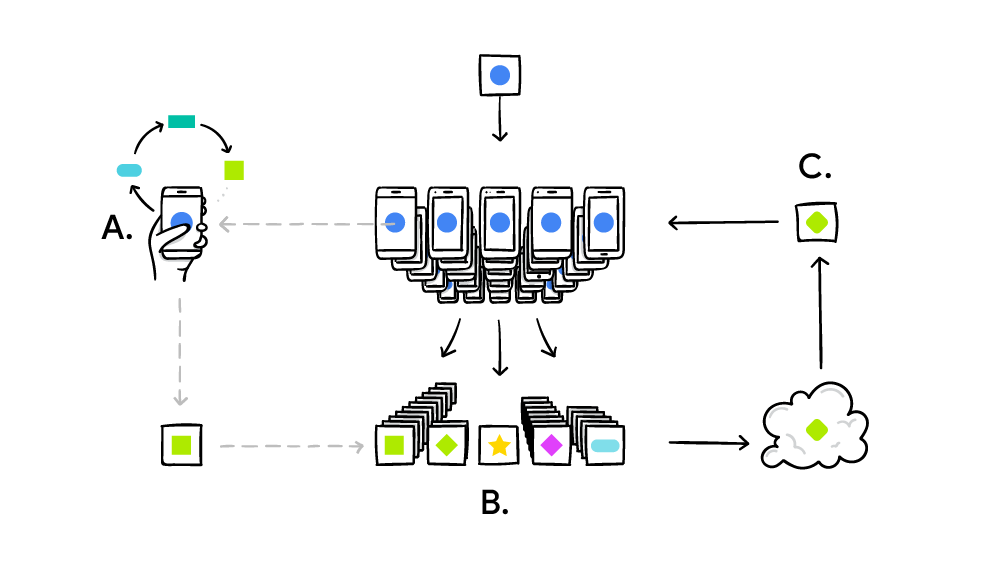
\includegraphics[width = \linewidth]{fig/FederatedLearningFlow}
\caption{联合学习流程图:A 根据手机的使用情况,对本地模型进行个性化设置并训练上传模型更新;B 许多用户的模型更新被聚集在一起;C 优化共享模型,然后很多用户又对新的模型进行下载、训练,并重复这个过程。}
\label{fig:Google}
\end{figure*}

\section{相关工作}
\subsection{基于差分隐私的协作学习}
在\cite{shokri2015privacy}提出的协作学习中,通过采用选择参数分享(Selective Parameter Sharing)使得用户可以有选择性地分享模型参数,以保证用户的数据不被泄露,在可用性和隐私之间tradeoff。文中,Shokri等进一步提出,由于参数分享过程可能会有非常少的一部分数据会被泄露,因此使用差分隐私的方式对分享的参数加入噪声(record-level),使得即使参数泄露也不会对用户的隐私数据造成威胁。当差分隐私中的$\epsilon$越小时(表示更强的隐私保护)将会导致模型的Accuracy降低,因此这种方式是在模型的准确性(Accuracy)和隐私之间tradeoff。实验结果如图3所示。

\begin{figure*}[!ht]
\begin{tabular}{ccc}
\subfloat[参与者为30人]{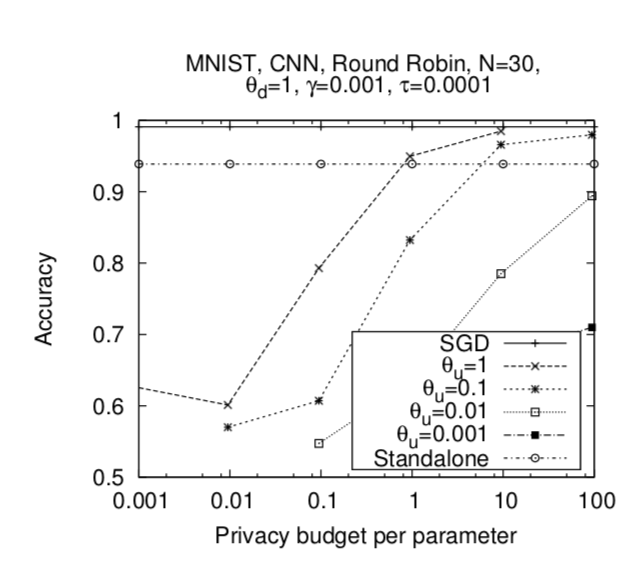
\includegraphics[width = 2in]{fig/ccs15_1}}&
\subfloat[参与者为90人]{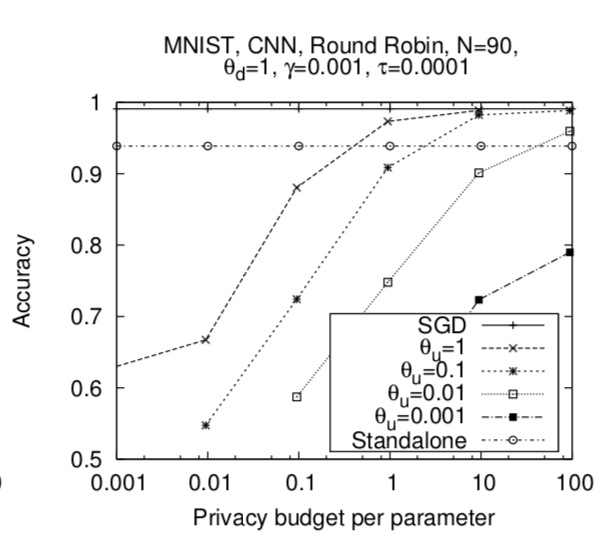
\includegraphics[width = 2in]{fig/ccs15_2}}&
\subfloat[参与者为150人]{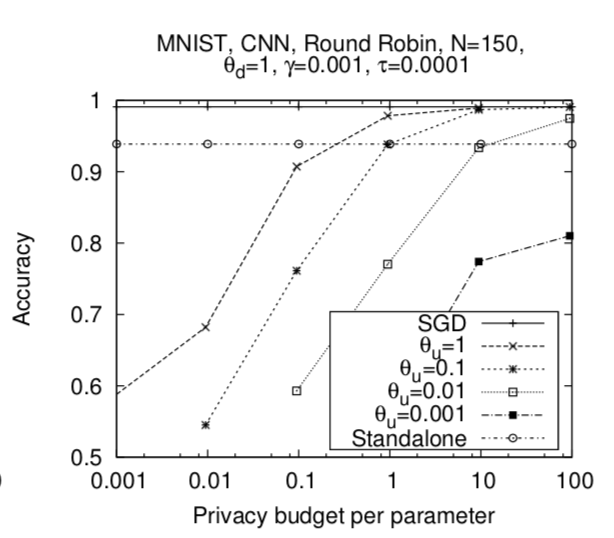
\includegraphics[width = 2in]{fig/ccs15_3}}
\end{tabular}
\caption{在MNIST数据集上,对CNN网络的含有差分隐私的协作学习。其中横轴为$\epsilon$,表示差分隐私的强度$\epsilon$越大差分隐私保护添加的噪声越弱。N表示参与者的人数,$\theta_d$表示参数下载的比例,$\theta_u$表示参数上传到比例。从图中可以看出,1:条件相同时参与人数越多准确性越高;2:$\epsilon$越大(噪声越小)准确性越高;3:$\theta_u$越大准确性越高。}
\label{fig:CCS15}
\end{figure*}


\subsection{基于同态加密的协作学习}
2017年,Phong等人在TIFS'17上发表了文章\cite{Phong2017PrivacyPreservingDL},对\cite{shokri2015privacy}提出的协作学习模型的安全及隐私性进行分析,并提出使用同态加密的方法来加密上传给服务器的梯度(gradients)。而且,为了进一步确保在上传给服务器的同态加密密文的完整性,在于服务器的通讯中采用TLS/SSL安全信道。Phong等人假定协作学习中的PS服务器是半可信(honest but curious)的,在参与者上传参数时,服务器是好奇的,在执行协议操作时,服务器是诚实的。一方面,对需要上传到服务器上的梯度使用基于LWE或者Paillier的同态加密会增加参与者与服务器之间的通讯开销,但实验表明增加的通讯开销量还是可接受的;另一方面,对于需要上传到梯度使用同态加密计算会增加一部分计算量,但相比于\cite{shokri2015privacy}中使用差分隐私减少了一部分准确性来说,计算量的增加带来效率的降低还是可以接受的,因为毕竟在深度学习领域准确性一定比效率更重要。相关过程如图4所示。

\begin{figure*}[!ht]
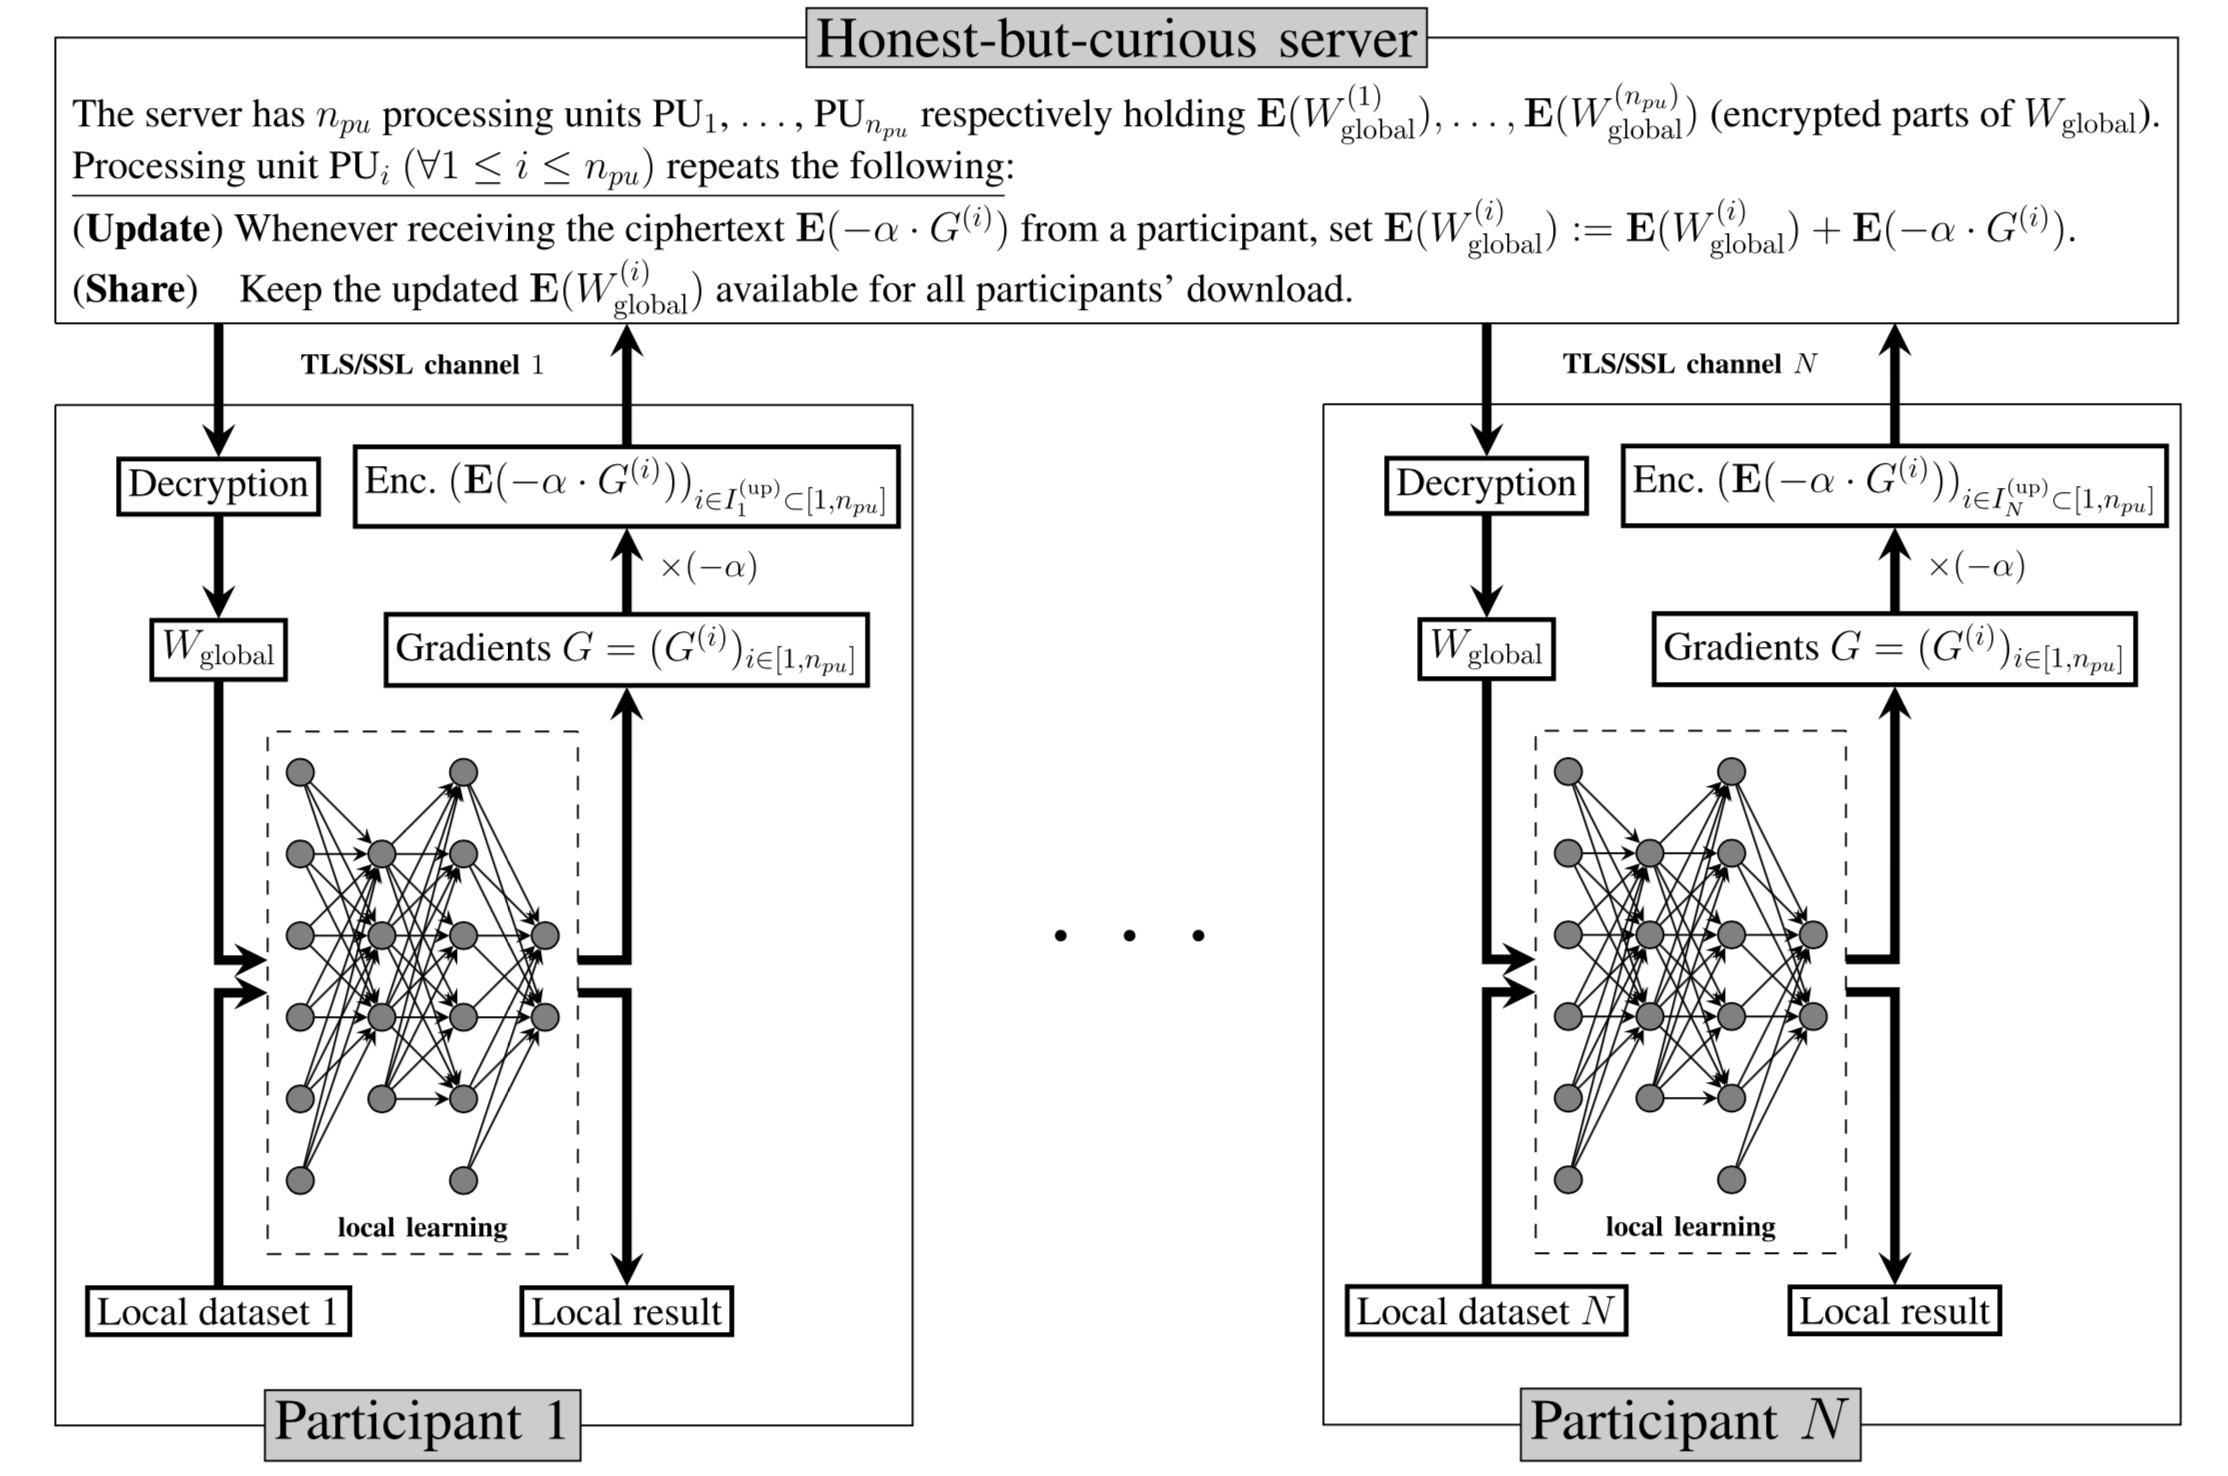
\includegraphics[width = \linewidth]{fig/TIFS17.png}
\caption{使用同态加密的协作学习模型}
\label{fig:TIFS17}
\end{figure*}

\subsection{对协作学习模型的攻击}
\subsubsection{介绍}
和\cite{Phong2017PrivacyPreservingDL}考虑的服务器对参与者训练数据
\cite{shokri2015privacy}和\cite{Phong2017PrivacyPreservingDL}中都是假定服务器是半可信的,考虑的都是服务器有可能会窃取参与者的训练数据。而Hitaj等人在CCS'17上发表了一篇关于协作学习中参与者隐私泄露的文章\cite{hitaj2017deep},考虑的是参与者有可能是active的Adversary,从而获取到其他参与者的训练数据。文章\cite{hitaj2017deep}对\cite{shokri2015privacy}中提出的协作学习进行了攻击,通过使用对抗生成网络(GAN)成功地从其中某个参与者中获得了训练数据。进一步地,即使在将参数上传至服务器之前使用差分隐私在参数中加入噪声,只要差分隐私的粒度是record-level的,攻击仍然可以成功。不同于模型训练完后对模型进行攻击的黑盒攻击,如model extraction attacks;Model inversion attacks;Membership inference attacks,这是一种在训练阶段发生的白盒攻击,在这种攻击中攻击者像其他参与者一样参与到模型的训练中,可以看到并使用模型的参数。但是,在这种攻击中,攻击者会偷偷地使用其他参与者共享的参数使用GAN网络生成与受害者训练数据类似的数据,每一次迭代攻击者都可以获取到更多受害者的训练数据,最后攻击者可以完整的还原出受害者的训练数据,攻击成功。在这种情况下,只要参与者的本地模型精确度足够高,攻击者都可以成功获取到受害者的原始训练数据。


值得一提的是,\cite{hitaj2017deep}提出的这种攻击方法对于Google的联合学习模型同样有用。和\cite{shokri2015privacy}使用差分隐私来保护分享的参数不同,联合学习中采用了一种安全聚集协议(secure aggregation protocol)\cite{bonawitz2017practical}。通过使用安全多方计算(MPC)去计算模型参数的平均权重,根据这个权重每个移动设备的更新(updates)都可以被安全地聚集起来,而且这也使得只有在多个用户的参与下Google才能对模型参数进行解密,这样就可以防止Google窃取用户的模型参数。由于\cite{bonawitz2017practical}的安全模型中只考虑了Google可能是Adversary,并没有考虑到\cite{hitaj2017deep}中提出的参与者的任何一个人都可能成为Adversary,进而去攻击其他参与者以获取其训练数据。


\subsubsection{威胁模型}
如\cite{shokri2015privacy}中所说,协作学习中,所有的参与者会提前对共同的学习目标达成一致。这就意味着,Adversary已经可以知道模型的结构和所有其他参与者的标签了。设$V$为受害者并且有标签$[a,b]$,$A$为敌手且有标签$[b,c]$。$A$的目标就是尽可能推断出更多关于$a$的信息。$A$会使用GAN生成非常类似$a$的样本,然后把它标记成$c$,并在本地训练,并将其模型参数上传至服务器。这样,$V$需要去在$a$和$c$中辨别真假,就会暴露更多关于$a$的信息。详细步骤如下:
\begin{enumerate}
\item 假设$A$和$V$双方提前对学习结构和目标达成了一致。
\item $V$有标签$[a,b]$,$A$有标签$[b,c]$。
\item 执行协作深度学习协议若干轮,当且仅当参数服务器上的模型和本地的模型都达到特定的准确度才停止迭代。
\item $V$开始训练:
	\begin{enumerate}
	\item $V$从参数服务器上下载部分参数($\theta_d$),并更新本地模型。
	\item $V$在$[a,b]$上训练本地模型。
	\item $V$上传部分本地模型的参数到服务器上。
	\end{enumerate}
\item $A$开始训练:
	\begin{enumerate}
	\item $A$从参数服务器上下载部分参数($\theta_d$),并更新本地模型。
	\item $A$训练本地的GAN来模仿$V$的$a$。
	\item $A$的GAN生成样本,并把它们标记成$c$。
	\item $A$在$[b,c]$上训练本地模型。
	\item $A$上传部分本地模型的参数到服务器上。
	\end{enumerate}
\item 重复步骤4和5,直到模型收敛。
\end{enumerate}
攻击过程如图\ref*{fig:ganscenario}所示。

\begin{figure*}[!ht]
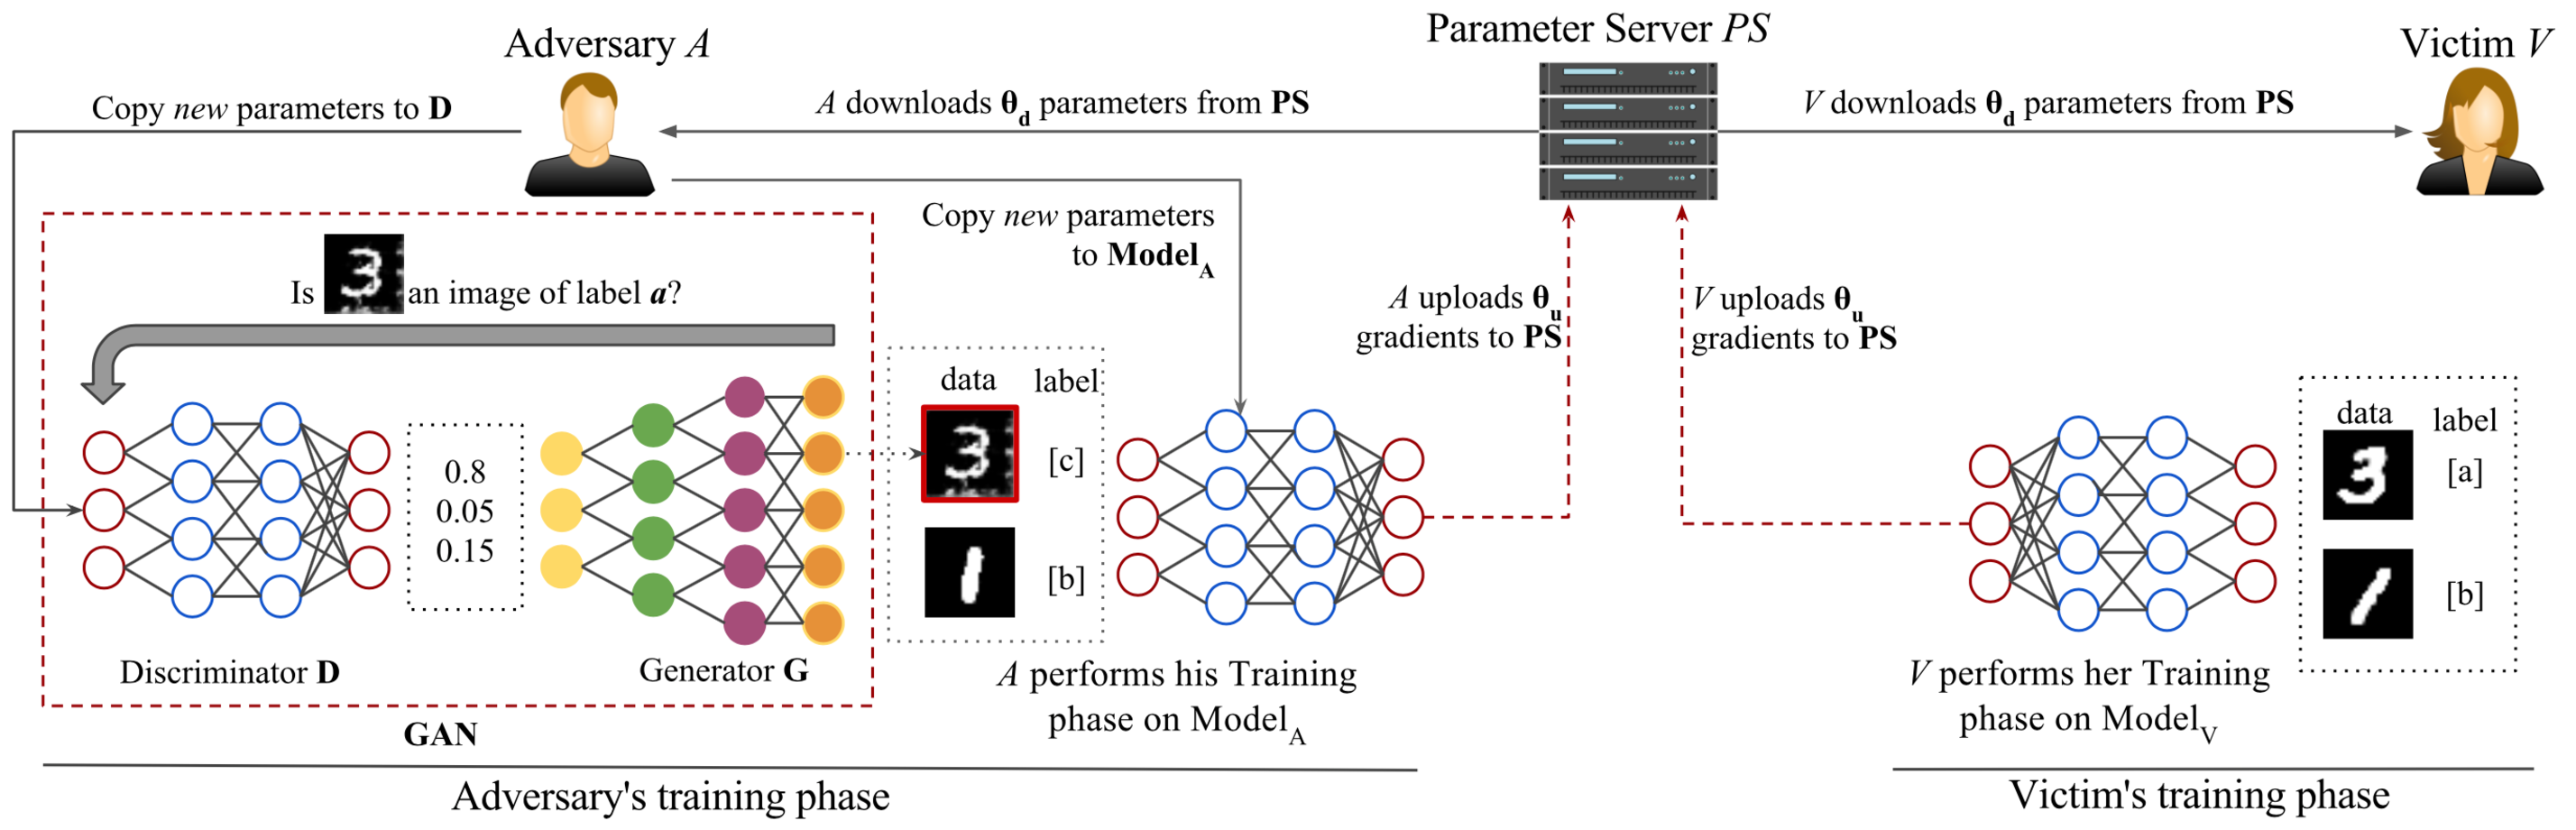
\includegraphics[width = \linewidth]{fig/ganscenario_new.pdf}
\caption{使用GAN攻击正在训练MNIST数据集的协作深度学习模型。}
\label{fig:ganscenario}
\end{figure*}

\subsubsection{实验结果}
实验采用MNIST和来自AT\&T的Olivetti人脸数据集,使用DCGAN攻击,并分别就有无使用差分隐私对照试验。实验结果如图\ref*{fig:ganresults}和图\ref*{fig:41_participants}所示。

\begin{figure*}[!ht]
\centering
\setlength{\tabcolsep}{2pt}
\begin{tabular*}{\textwidth}{c c c}
\setlength{\tabcolsep}{1pt}
\subfloat[$\theta_u = 1, \theta_d = 1$]{
\begin{tabular}{lllll}

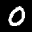
\includegraphics[width = 0.4in]{fig/original_for_sample_5_400_100.png}  & 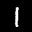
\includegraphics[width = 0.4in]{fig/original_for_sample_5_390_200.png} & 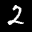
\includegraphics[width = 0.4in]{fig/original_for_sample_5_500_300.png} & 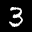
\includegraphics[width = 0.4in]{fig/original_for_sample_5_480_400.png} & 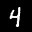
\includegraphics[width = 0.4in]{fig/original_for_sample_5_400_500.png} \\ 
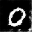
\includegraphics[width = 0.4in]{fig/sample_5_epoch_400_taskid_100.png}  & 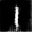
\includegraphics[width = 0.4in]{fig/sample_5_epoch_390_taskid_200.png} & 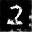
\includegraphics[width = 0.4in]{fig/sample_5_epoch_500_taskid_300.png} & 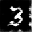
\includegraphics[width = 0.4in]{fig/sample_5_epoch_480_taskid_400.png} & 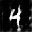
\includegraphics[width = 0.4in]{fig/sample_5_epoch_400_taskid_500.png}  \\
\end{tabular}
}
    &
 \setlength{\tabcolsep}{1pt}
\subfloat[$\theta_u = 0.1, \theta_d = 1$]{
\begin{tabular}{lllll}


\includegraphics[width = 0.4in]{fig/original_for_sample_4_950_0.png}  & 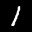
\includegraphics[width = 0.4in]{fig/original_for_sample_4_960_1.png} & 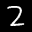
\includegraphics[width = 0.4in]{fig/original_for_sample_5_910_3.png} & 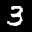
\includegraphics[width = 0.4in]{fig/original_for_sample_5_870_4.png} & 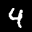
\includegraphics[width = 0.4in]{fig/original_for_sample_5_830_5.png} \\ 
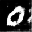
\includegraphics[width = 0.4in]{fig/sample_4_epoch_950_taskid_0.png}  & 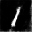
\includegraphics[width = 0.4in]{fig/sample_4_epoch_960_taskid_1.png} & 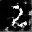
\includegraphics[width = 0.4in]{fig/sample_5_epoch_910_taskid_3.png} & 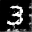
\includegraphics[width = 0.4in]{fig/sample_5_epoch_870_taskid_4.png} & 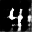
\includegraphics[width = 0.4in]{fig/sample_5_epoch_830_taskid_5.png} \\ 
\end{tabular}
}
    &
 \setlength{\tabcolsep}{1pt}
\subfloat[$\theta_u = 0.1, \theta_d = 0.1$]{
\begin{tabular}{lllll}


\includegraphics[width = 0.4in]{fig/original_for_sample_4_1650_100.png}  & 
\includegraphics[width = 0.4in]{fig/original_for_4_1610_200.png} & 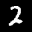
\includegraphics[width = 0.4in]{fig/original_for_4_1620_300.png} & 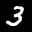
\includegraphics[width = 0.4in]{fig/original_for_sample_4_1620_400.png} & 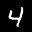
\includegraphics[width = 0.4in]{fig/original_for_sample_5_1950_500.png}\\ 
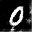
\includegraphics[width = 0.4in]{fig/sample_4_epoch_1650_taskid_100.png}  & 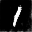
\includegraphics[width = 0.4in]{fig/sample_4_epoch_1610_taskid_200.png} & 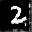
\includegraphics[width = 0.4in]{fig/sample_4_epoch_1620_taskid_300.png} & 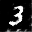
\includegraphics[width = 0.4in]{fig/sample_4_epoch_1620_taskid_400.png} & 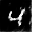
\includegraphics[width = 0.4in]{fig/sample_5_epoch_1950_taskid_500.png} \\ 
\end{tabular}
}
\end{tabular*}
\caption{使用GAN在MNIST数据集上攻击两个参与者场景下的结果。图中下面一行是GAN生成的样本,上面一行是受害者训练集中的数据。}
\label{fig:ganresults}
\end{figure*}


\begin{figure*}[!ht]
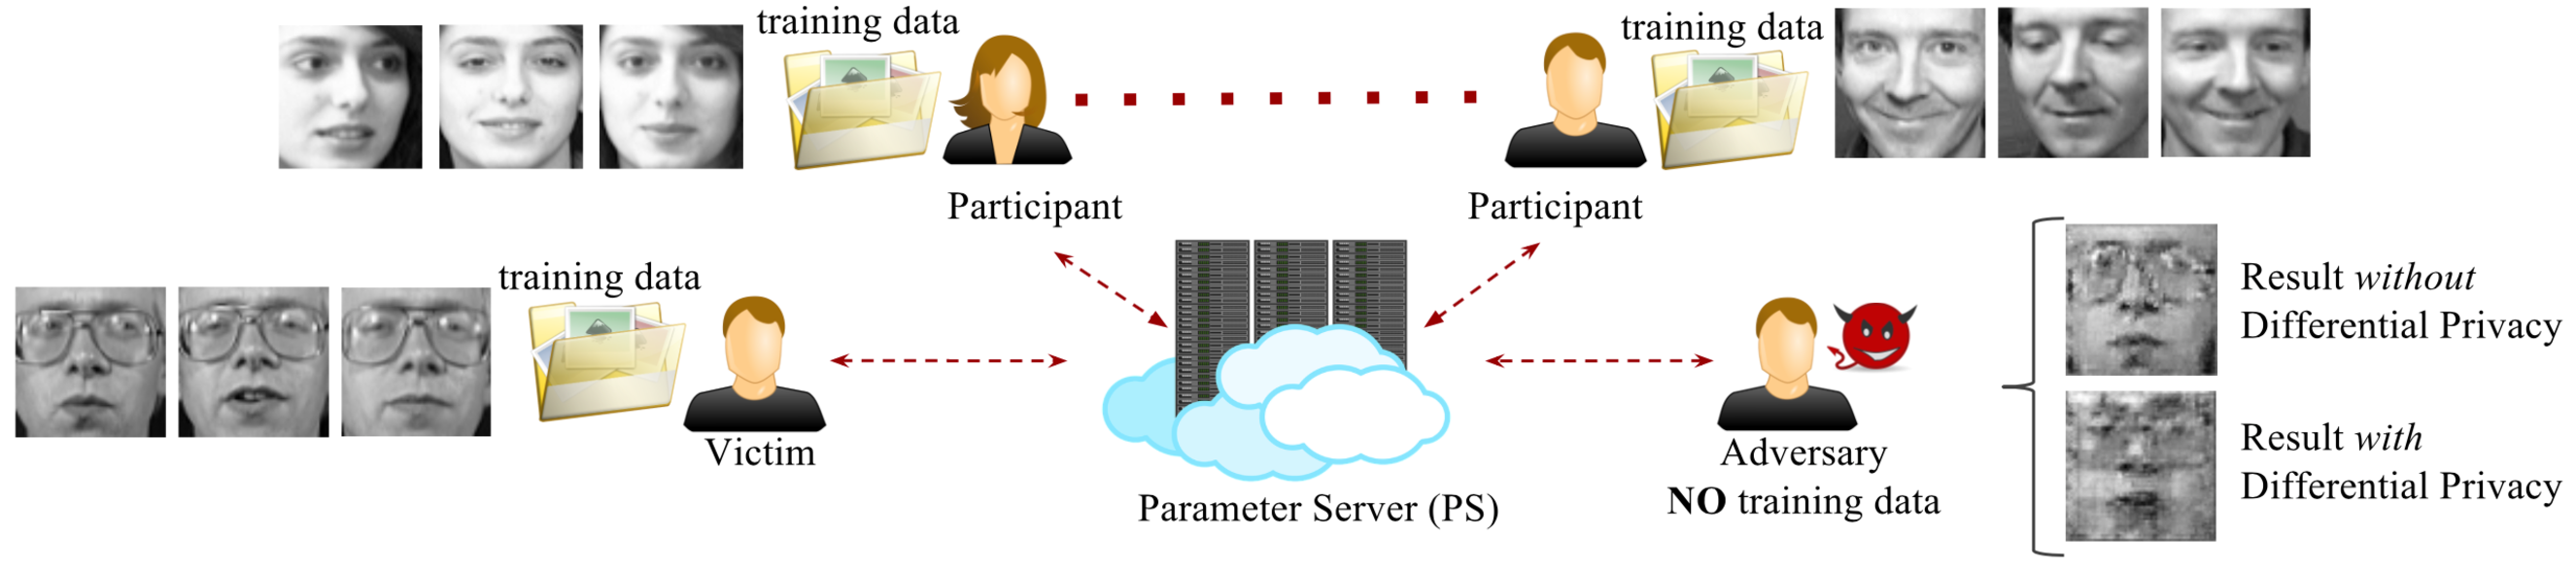
\includegraphics[width = \linewidth]{fig/41_participants.pdf}
\caption{使用GAN在AT\&T的Olivetti人脸数据集上攻击的结果。诚实的参与者们互相独立地训练模型,且敌手$A$并没有本地的训练数据,通过使用GAN攻击,$A$可以重新构建出受害者$V$的训练数据。即使在使用差分隐私的情况下,这种攻击也能成功。}
\label{fig:41_participants}
\end{figure*}


\section{想法及未来工作}
因为刚接触深度学习及其隐私问题不久,可能对其了解不够深刻。我想以此工作作为切入点,继续再次详细地看一看本文涉及的paper。一方面持续关注深度学习领域的隐私保护问题,另一方面还要看看目前比较热门的基因技术和机器学习技术的结合点及其隐私保护问题,或者是否可以根据基因数据的特点,将现有的机器学习的隐私保护方案用到基因数据的隐私保护方面。

\bibliographystyle{IEEEtran}
\bibliography{references}
\end{document}


















